% Generated by pysimcount.pfboundratio -- do not edit; regenerate instead.
% figure: bound-ratio-suzuki8 -- Suzuki S8: Trotter number from each bound / measured r, against n
% metric=r_ratio gatebase=cz; geometric mean over seeds [1, 2, 3, 4, 5, 6, 7, 8, 9, 10], bars min-max; r_method=measured (denominator); bounds: Analytic bound, Minimised bound, Commutator bound (2018), Commutator bound (2021), Empirical fit (2018)
% sizes: np-main n = [4, 5, 6, 7, 8, 10]; np-main-n9 n = [9]; np-main-n11 n = [11]
% run set np-main-n9 made from uncommitted code (git_dirty), accepted: run at e42ff29 with the only modified tracked file pysimcount/pfseeds.py (an aggregation module the run does not import); checked with git diff --stat e42ff29 -- pysimcount/ on 2026-11-08
% run set np-main-n11 made from uncommitted code (git_dirty), accepted: run at e42ff29 with the only modified tracked file pysimcount/pfseeds.py (an aggregation module the run does not import); checked with git diff --stat e42ff29 -- pysimcount/ on 2026-11-08
% formulas: Suzuki S8
% figure made at git_commit=e5d9ee696f892e28aced765585653760f8a427c4 git_dirty=False
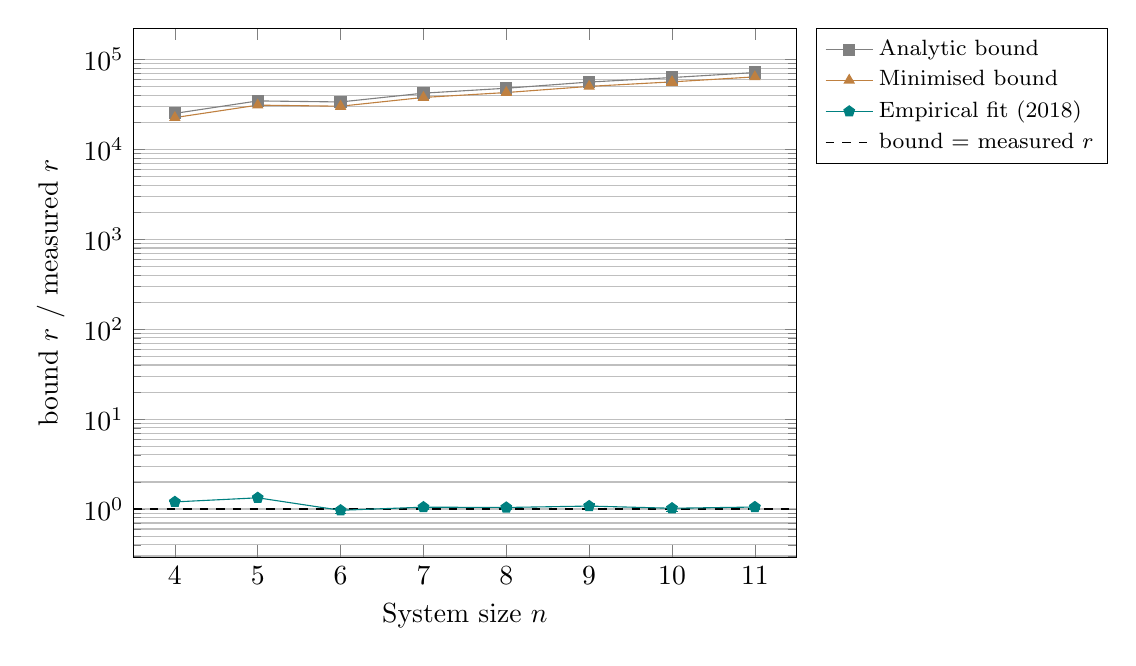
\begin{tikzpicture}
  \begin{semilogyaxis}[
    width=10cm, height=8.3cm,
    xlabel={System size $n$}, ylabel={bound $r$ / measured $r$},
    xmin=3.5, xmax=11.5,
    xtick={4,5,6,7,8,9,10,11},
    ymajorgrids=true, yminorgrids=true,
    legend pos=outer north east, legend cell align=left,
    legend style={font=\footnotesize},
  ]
    \addplot[dashed, black, domain=3.5:11.5, samples=2, forget plot] {1};
    \addplot[solid, gray, mark=square*, mark size=2pt, error bars/.cd, y dir=both, y explicit] coordinates {
      (4,25137) -= (0,3.63798e-12) += (0,-3.63798e-12)
      (5,34608.2) -= (0,0) += (0,0)
      (6,33691.3) -= (0,2395.39) += (0,1081.93)
      (7,42210.6) -= (0,1964.37) += (0,2060.25)
      (8,47867.1) -= (0,1877.88) += (0,1954.56)
      (9,56076.8) -= (0,414.037) += (0,3867.71)
      (10,62965.9) -= (0,4862.99) += (0,2884.07)
      (11,71589.5) -= (0,3589.62) += (0,410.366)
    };
    \addlegendentry{Analytic bound}
    \addplot[solid, brown, mark=triangle*, mark size=2pt, error bars/.cd, y dir=both, y explicit] coordinates {
      (4,22579.8) -= (0,-1.45519e-11) += (0,1.45519e-11)
      (5,31058.2) -= (0,-2.18279e-11) += (0,2.18279e-11)
      (6,30213.1) -= (0,2148.1) += (0,970.233)
      (7,37830.2) -= (0,1760.52) += (0,1846.45)
      (8,42878.3) -= (0,1682.16) += (0,1750.85)
      (9,50210.9) -= (0,370.728) += (0,3463.13)
      (10,56358.4) -= (0,4352.68) += (0,2581.42)
      (11,64056.1) -= (0,3211.89) += (0,367.183)
    };
    \addlegendentry{Minimised bound}
    \addplot[solid, teal, mark=pentagon*, mark size=2pt, error bars/.cd, y dir=both, y explicit] coordinates {
      (4,1.2) -= (0,0) += (0,0)
      (5,1.33333) -= (0,0) += (0,0)
      (6,0.968886) -= (0,0.0688862) += (0,0.0311138)
      (7,1.04881) -= (0,0.0488088) += (0,0.0511912)
      (8,1.04083) -= (0,0.040833) += (0,0.0425003)
      (9,1.0794) -= (0,0.00796963) += (0,0.0744479)
      (10,1.01995) -= (0,0.0787729) += (0,0.0467173)
      (11,1.05279) -= (0,0.0527887) += (0,0.0060348)
    };
    \addlegendentry{Empirical fit (2018)}
    \addlegendimage{dashed, black}
    \addlegendentry{bound $=$ measured $r$}
  \end{semilogyaxis}
\end{tikzpicture}
